\section{Assoliment dels objectius}

\subsection{Estudi de l'estat de l'art}
S'ha realitzat un estudi extens de l'estat de l'art, que ha requerit diverses setmanes de recerca i estudi dels avenços més nous en la matèria. S'ha pogut veure com aquest camp avança a un pas imparable i on pràcticament setmanalment apareixen noves solucions per provar. Tant a l'espai \textit{open source} com al privat, s'ha pogut posar a prova les tecnologies més modernes disponibles i valorar els seus avantatges i desavantatges. Es considera que aquest objectiu \textbf{ha sigut assolit satisfactòriament}.

\subsection{Extracció tiquets d'una base de dades OTRS}
S'ha estudiat i comprès el funcionament intern del sistema de tiquets \textit{OTRS} i la llibreria \textit{PyOTRS} i per aconseguir configurar una base de dades amb aquest sistema i extreure els tiquets amb tota la informació necessària. S'ha dissenyat un sistema per poder obtenir tiquets específics de base de dades tenint en compte les limitacions de l'entorn en el qual es treballava. El sistema d'extracció de tiquets permet una gran flexibilitat per rebre tiquets en diferents formats o amb diferents continguts en cas que sigui necessari una modificació o ampliació futura. Es considera que aquest objectiu \textbf{ha sigut assolit satisfactòriament}.

\subsection{Preprocessament del text d'entrada}
El text dels tiquets ha sigut processat primerament per obtenir el text sense format i després per eliminar tot el contingut redundant o innecessari possible. S'ha dissenyat i entrenat diversos models d'eliminació de signatures amb conceptualment diferents encara que no han sigut implementades a la solució final. Es considera que aquest objectiu \textbf{ha sigut assolit satisfactòriament}.

\subsection{\textit{Fine-tune} d'un model de \textit{Deep learning}}
Gràcies a la recerca inicial i la continuada durant el progrés del projecte, s'ha provat, entrenat i validat diversos models de \textit{Deep learning} amb l'objectiu d'extreure els camps especificats. S'ha aconseguit entrenar un model que obté un 71,4\% d'encerts en les proves de validació. Es considera que aquest objectiu \textbf{ha sigut assolit satisfactòriament}.

\subsection{Anonimització de la sortida del sistema}
S'ha instal·lat i configurat \textit{Logstash} per rebre la sortida del model d'extracció d'informació en format JSON. S'ha desenvolupat una funció que anonimitza cada camp depenent del seu tipus i reparteix segons la seva destinació. Aquesta funció es pot parametritzar per a rebre més camps dels especificats. Es considera que aquest objectiu \textbf{ha sigut assolit satisfactòriament}.

\subsection{Emmagatzematge de les dades en Elasticsearch}
En conjunció amb el mòdul de Logstash, s'ha instal·lat i configurat una base de dades \textit{Elasticsearch}. Es pot inserir en dos índexos diferents el resultat anonimitzat rebut del mòdul de \textit{Logstash}. Es considera que aquest objectiu \textbf{ha sigut assolit satisfactòriament}.

\subsection{Implementació del pipeline}
El \textit{pipeline} ha sigut dissenyat i implementat des de zero, tenint en compte les especificacions i limitacions del projecte. La figura \ref{fig:pipeline_flux_real} il·lustra el desplegament final de la \textit{pipeline}. Es pot veure com el portàtil amb GPU només s'utilitza per a l'execució del model, però la resta d'eines s'executen en el seu servidor designat. Es considera que aquest objectiu \textbf{ha sigut assolit satisfactòriament}.

\begin{figure}[H]
\centering
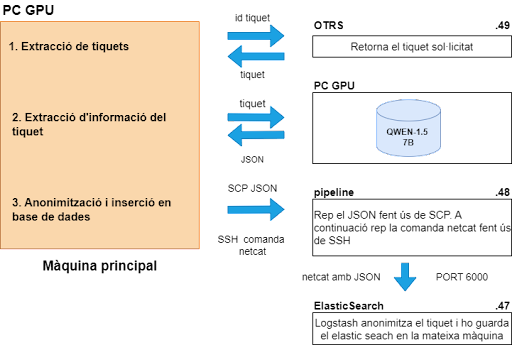
\includegraphics[width=\textwidth]{pipeline_flux_real.png}
\caption[\textit{Pipeline} mostra el flux d'execució final]{\textit{Pipeline} que mostra el flux d'execució final fent servir el portàtil amb GPU. \\ (Creació pròpia)}
\label{fig:pipeline_flux_real}
\end{figure}

\subsection{Desplegament API}
L'API implementada disposa de dos \textit{endpoints} senzills. El primer només accepta un número de tiquet com a entrada. El segon espera un fitxer Excel que conté una llista de números de tiquets i el \textit{pipeline} processa cadascun individualment. Es considera que aquest objectiu \textbf{ha sigut assolit satisfactòriament}.